%
\section{Testing}
%
test site can be found at thesis.fmitcar.appspot.com/thesis/start/
%
\subsection{Test Environment}
%

%
All our video summaries are hosted on YouTube.
%
\subsubsection{Questionnaire}
%
% reverse engineer questions (find lit. on how to write a questionnaire)
%
The questionnaire was structured as a statement and 5 options
%
% Noter fra Kim: Vis figur med spørgsmål ANDERS: DE STÅR JO LIGE NEDE UNDER (begin itemize)
%
where the test user could either agree, disagree, or indicate that they were unable to respond to the statement. An example of a statement was INSERT STATEMENT HERE and the possible replies was Totally agree, Somewhat agree, Somewhat disagree, Totally disagree, and Don't know, in that order. We initially had "dont't know" in the middle, but we learned from a test-run of our questionnaire that placing it last would result in a higher rate of usable responses.\\
%
% Noter fra Kim: Har i så smidt resultater væk? LAUGE
%
% Noter fra Lauge: Bør vi nok fjerne. Ikke super relevant. JO I HØJ GRAD RELEVANT.
%
%
We want to investigate a few crucial points in depth which resulted in 4 very different statements:
%
\begin{itemize}
\item The individual video clips are interesting
\item The video is well edited
\item The length of the individual video clips are fitting
\item The length of the entire video is fitting
\end{itemize}
%
The first statement investigates the quality of our labeller. The second statement investigates how well we are able to combine segments (in other words the quality of our recipe, ie. the order and context of the ingredients). The third statement investigates the general attitude towards clip-length, which is chosen somewhat at random within boundaries determined by the recipe. The fourth statement investigates the general attitude towards the total length of a video-summary. The ordering of statements changes between asking to the enterity of the video to each individual clip.\\
We also added an optional note to each questionnaire in case a user wanted to ellaborate on their answer(s).
%
\subsubsection{Setup}
%
As we both have a good deal of experience with \textit{Google App Engine} we choose to deploy a small website where our test panel could rate video-summaries.\\%We used a spartan styling of the site such as a white background.
%
% Noter fra Kim: What?
%
% Noter fra Lauge: Minimalistic? 
%
%
To discern interuptive elements we removed player-controls from the YouTube embedded player (the user could still pause the video by clicking on it or using the space-bar on their keyboard), and also disable the recommended videos that appear after playing a YouTube video to the end. The questionnaire was not shown before the end of the video in order not to disctract attention to it. The video-title, which would appear briefly in the top of the player was the hex-value of a randomly generated number to ensure a non-descript title.\\
We supplied each session with a unique identifier. This means that we are unable to track a returning test-user, as they would get a new session id, but it does give us a rough measure of how many different test-users we get, how many questionnaires answered on average, and also investigate the progress of a test-user (they may generally rate a video worse as they watch more videos) - the time at which a result is recorded is saved along with the data.\\
To increase the availability of our test environment everything is localized into danish and english - especially elderly danish people may have a hard time answering an english questionnaire.
%
% Noter fra Kim: Hvad er de danske oversættelser? De skal angives LAUGE
%
The resulting locale is recorded along with each result. This will also allow us to measure any significant difference between the two locales - as it is impossible to make a 1-to-1 translation of the statements.\\
To ensure a proper shuffling of each video-summary we record how many times a given summary is shown (it counts as shown when a test-user has completed the questionnaire). We consequently enforce a balance of this counter amongst all the videoes. Furthermore we restrict, if possible, that a video has not been shown recently (within the last 3 minutes). This would allow us to easily add more videos later on should the need arise, while getting results from the entire range of summaries.\\
%
% Noter fra Kim: Det forstår jeg ikke
%
% Noter fra Lauge: Det er heller ikke helt tilfældet som vi også sidenhen snakkede om. LAUGE
%
%
We initially spread the survey on Facebook by messaging friends and family and making a public wall post. To further increase the chance of the survey going viral we placed a Facebook Like-button and a Twitter button discretely in the bottom of the site to allow test-users to further spread the word.\\
We designed the test so that the test-user can watch as many or as few videos as they want, ie. each video-summary is a self-contained questionnaire.
%
\subsubsection{Control Samples}
%
%
\subsubsection{Random Segments}
% 
For each dataset we created a videoclip totally at random, ie. we picked a random video, and a random segment within that video, and cut it all together. The segment length was chosen such that they would not differ significanytly from the general length of other computer generated videoclips. These videoclips are thought of as a baseline (we expect them to perform poorly compared to even random labels recipe).
%
\subsubsection{Human Edited}
% 
We used humanly edited videoclips as a control sample. A select few videos was cut to fit the general length of other computer generated videoclips.
%
% Noter fra Kim: Hvor kommer de fra?
%
We add two different control samples: one is videos with a random set of labels and segment lengths, and one where clips was picked totally at random.
%
% Noter fra Kim: See section XX WOOOOT??? ANDERS
%
This will form the baseline for our test, ie. we expect these to perform poorly in all aspects. We also added videos edited by humans as a control sample. We expect these to perform as well as the designer recipies or better.
%
\subsection{Results}
%
The first step in our analysis of the collected data is to plot histograms of the answers in each method, as seen in Figure \ref{fig:hist_design} (additional figures can be found in Appendix \ref{app:histograms}), in order to investigate the distribution of answers. As see in Figure \ref{fig:hist_design} the answers are unevenly distributed with a skew to the right with the exception of the first histogram (content). The answers are generally unevenly distributed in the other histograms which allows us to continue our analysis. Had there been a trend of an even distribution of answers the data would have been inconclusive by definition.
%
\begin{figure}
     \centering
     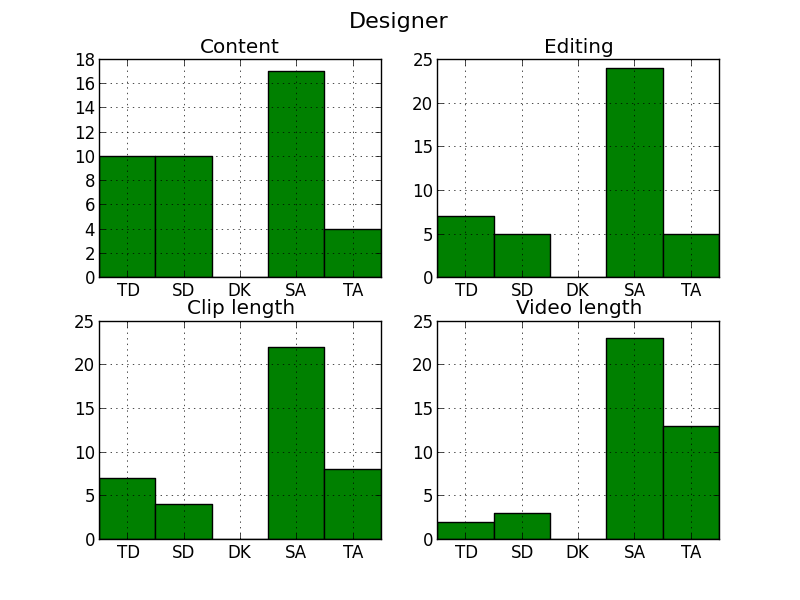
\includegraphics[width=1.0\textwidth]{img/designer_barplot.png}
     \caption{Histogram of answers to videos created with the "designer method"}\label{fig:hist_design}
\end{figure}
%
We continue our analysis by employing the Friedman test\footnote{http://en.wikipedia.org/wiki/Friedman\_test} which is a non-parametric statistical test (we make no assumptions on the normality of our data). The results can be found in Tables \ref{tab:fried_alpha}, \ref{tab:fried_dataset}, and \ref{tab:fried_recip}. 
%
\begin{table}[ht]
	\begin{center}
	\caption{Friedman rank sum test for recipies}
	\label{tab:fried_recip}
		\begin{tabular}{lccc}
		\toprule
			 & v & p-value & $x^2$\\
			\midrule
			Content & $3$ & $0.3242$ & $3.4737$\\
			Editing & $3$ & $0.3260$ & $3.4602$\\
			Clip length & $3$ & $0.9597$ & $0.3016$\\
			Video length & $3$ & $0.3218$ & $3.4918$\\
			Total score & $3$ & $0.4882$ & $2.4292$\\
		\bottomrule
		\end{tabular}
	\end{center}
\end{table}
\begin{table}[ht]
	\begin{center}
	\caption{Friedman rank sum test for datasets}
	\label{tab:fried_dataset}
		\begin{tabular}{lccc}
		\toprule
			 & v & p-value & $x^2$\\
			\midrule
			Content & $2$ & $0.0773$ & $5.1193$\\
			Editing & $2$ & $0.5436$ & $1.2190$\\
			Clip length & $2$ & $0.0577$ & $5.7059$\\
			Video length & $2$ & $0.2030$ & $3.1887$\\
			Total score & $2$ & $0.1185$ & $4.2656$\\
		\bottomrule
		\end{tabular}
	\end{center}
\end{table}
\begin{table}[ht]
	\begin{center}
	\caption{Friedman rank sum test for $\alpha$-span}
	\label{tab:fried_alpha}
		\begin{tabular}{lccc}
		\toprule
			 & v & p-value & $x^2$\\
			\midrule
			Content & $1$ & $0.7055$ & $0.1429$\\
			Editing & $1$ & $1.0000$ & $0.0000$\\
			Clip length & $1$ & $0.4652$ & $0.5333$\\
			Video length & $1$ & $0.7055$ & $0.1429$\\
			Total score & $1$ & $0.5271$ & $0.4000$\\
		\bottomrule
		\end{tabular}
	\end{center}
\end{table}
%
present notes + v = DoF, p-value, $x^2$ . hvad er i tables % ANDERS
%
\subsection{Analysis}
%
The only statistical significance is content in Table \ref{tab:fried_dataset}, which is no surprise as the datasets differ primarily on content as described in section \ref{section that describes datasets}. As everything else is statistically insignificant we do not pursue further analysis KIM: VI SKAL LIGE SNAKKE OM HVAD VI GØR HER.
%
\subsubsection{Risks \& Limitations}
%
% LAUGE
% hvad skal der stå her????
% limited dataset -> we did not have seperate training and test sets\\
% barely acceptable amount of feedback -> could have caused ...
% search keywrod kunne måske have hjulpet på at forstå spøgsmål bedre.
%
\subsection{Conclusion}
%
% ANDERS
%